% Work-MAT | 2. rocnik | hodina 13 | revize 2026-11-09
\documentclass[11pt,a4paper]{article}
\input{../../sablony/pripravy/priprava.sty}
\usepackage{tikz}
\usetikzlibrary{arrows.meta}
\nastavPripravu{2. ročník}{Exponenciální funkce}{13}{Exponenciální funkce III: grafy a transformace}
\begin{document}
\poznamka{Na začátku žáci samostatně narýsují do JEDNÉ soustavy grafy $y=2^x$ a $y=3^x$; využijí tabulku pro $x=-2,-1,0,1,2$. Diskutujte, co mají grafy společné a proč graf $3^x$ pro $x>0$ roste rychleji.}
\blok{Výchozí graf a jeho posuny}
V hodině 11 jsme zjistili, že základní exponenciální funkce $y=a^x$ prochází bodem $[0;1]$ a přibližuje se k ose $x$. Nyní využijeme znalost posunů grafů. Když předpis změníme na $g(x)=a^{x-p}+q$, neposunuje se jen graf, ale také jeho vodorovná asymptota. Nejprve si proto připravíme tabulku hodnot a několik význačných bodů.
\begin{zadaniBox}[title={Věta - Posuny exponenciálního grafu}]
Pro $a>0$, $a\ne1$ se graf $y=a^x$ převede na $g(x)=a^{x-p}+q$ posunutím podle pravidel
\[
\left\{\begin{aligned}
p:&\quad p>0\ \text{doprava},\quad p<0\ \text{doleva},\\
q:&\quad q>0\ \text{nahoru},\quad q<0\ \text{dolů}.
\end{aligned}\right.
\]
Vždy platí $D(g)=\mathbb R$, $H(g)=(q;+\infty)$ a vodorovná asymptota $y=q$.
\end{zadaniBox}
\begin{prikladReseniBox}[title={Příklad 1}]
Sestroj graf $g(x)=2^{x-1}+3$ a urči:
\begin{enumerate}[label=\alph*)]
\item posun vůči $2^x$;
\item $D(g)$, $H(g)$, asymptotu a monotónnost;
\item hodnoty $g(0)$, $g(1)$, $g(2)$.
\end{enumerate}
\tcblower
\begin{enumerate}[label=\alph*)]
\item Posun doprava o 1 a nahoru o 3.
\item $D(g)=\mathbb R$, $H(g)=(3;+\infty)$, asymptota $y=3$; roste.
\item $g(0)=\frac{7}{2}$, $g(1)=4$, $g(2)=5$.
\end{enumerate}\begin{center}
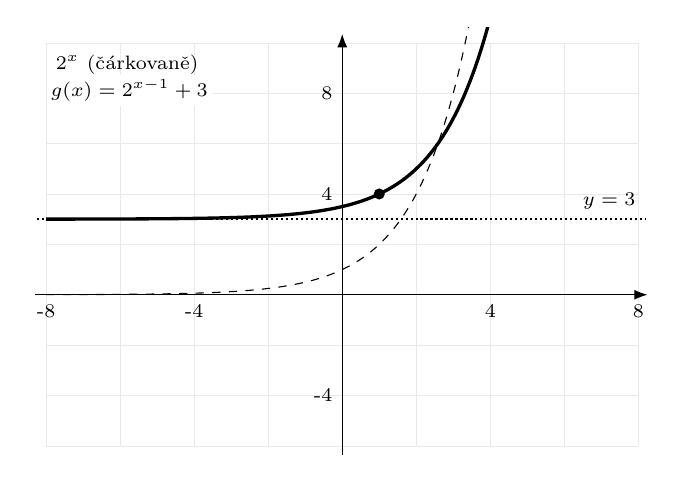
\begin{tikzpicture}[x=.47cm,y=.32cm,>=Latex]
\clip (-8.5,-6.5) rectangle (8.5,10.6);
\draw[step=2,gray!17,very thin] (-8,-6) grid (8,10);
\draw[->] (-8.3,0)--(8.25,0) node[right] {$x$};
\draw[->] (0,-6.35)--(0,10.35) node[above] {$y$};
\foreach \x in {-8,-4,4,8}{\node[below,font=\scriptsize] at (\x,0) {\x};}
\foreach \y in {-4,4,8}{\node[left,font=\scriptsize] at (0,\y) {\y};}
\draw[densely dotted,thick] (-8.25,3)--(8.2,3) node[above left,font=\scriptsize] {$y=3$};
\draw[thin,dashed,domain=-8:5,samples=110,smooth] plot (\x,{pow(2,\x)});
\node[font=\scriptsize,anchor=north west] at (-8,9.9) {{$2^x$ (čárkovaně)}};
\draw[very thick,domain=-8:5,samples=130,smooth] plot (\x,{pow(2,\x-1)+3});
\fill (1,4) circle (2pt);
\node[font=\scriptsize,anchor=north west,fill=white,inner sep=1.5pt] at (-8,8.75) {{$g(x)=2^{x-1}+3$}};
\end{tikzpicture}
\end{center}
\end{prikladReseniBox}
\blok{Zrcadlení a násobení funkčních hodnot}
Připojíme-li před kladnou exponenciálu záporné znaménko, graf se převrátí podle osy $x$. U obecnějšího předpisu $y=k\cdot a^{x-p}+q$ rozhoduje znaménko $k$ o tom, zda leží graf nad asymptotou, nebo pod ní. Číslo $q$ stále označuje výšku asymptoty.
\Needspace{25\baselineskip}
\begin{prikladReseniBox}[title={Příklad 2}]
Sestroj graf $h(x)=2-2^x$ a urči:
\begin{enumerate}[label=\alph*)]
\item vznik grafu ze základní funkce $2^x$;
\item $D(h)$, $H(h)$, asymptotu a monotónnost;
\item průsečíky s osami.
\end{enumerate}
\tcblower
\begin{enumerate}[label=\alph*)]
\item Převrácení podle osy $x$ a posun o 2 nahoru.
\item $D(h)=\mathbb R$, $H(h)=(-\infty;2)$; asymptota $y=2$, funkce klesá.
\item $h(0)=1$ dává bod $[0;1]$; $2^x=2$ dává bod $[1;0]$.
\end{enumerate}\begin{center}
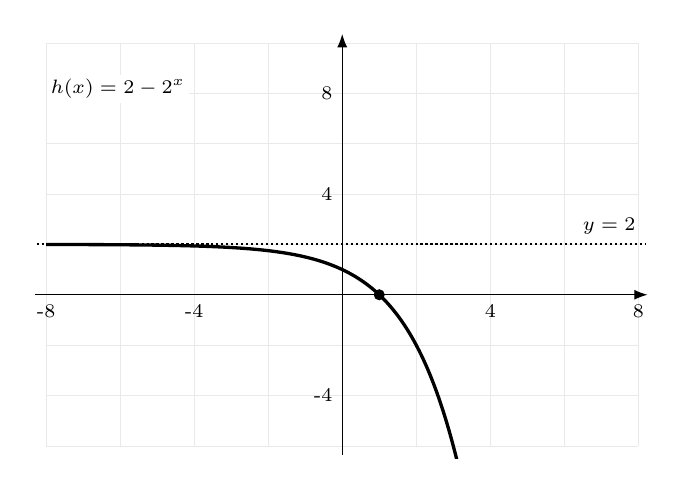
\begin{tikzpicture}[x=.47cm,y=.32cm,>=Latex]
\clip (-8.5,-6.5) rectangle (8.5,10.6);
\draw[step=2,gray!17,very thin] (-8,-6) grid (8,10);
\draw[->] (-8.3,0)--(8.25,0) node[right] {$x$};
\draw[->] (0,-6.35)--(0,10.35) node[above] {$y$};
\foreach \x in {-8,-4,4,8}{\node[below,font=\scriptsize] at (\x,0) {\x};}
\foreach \y in {-4,4,8}{\node[left,font=\scriptsize] at (0,\y) {\y};}
\draw[densely dotted,thick] (-8.25,2)--(8.2,2) node[above left,font=\scriptsize] {$y=2$};
\draw[very thick,domain=-8:5,samples=130,smooth] plot (\x,{2-pow(2,\x)});
\fill (1,0) circle (2pt);
\node[font=\scriptsize,anchor=north west,fill=white,inner sep=1.5pt] at (-8,8.75) {{$h(x)=2-2^x$}};
\end{tikzpicture}
\end{center}
\end{prikladReseniBox}
\begin{prikladReseniBox}[title={Příklad 3}]
Sestroj graf $k(x)=\left(\frac{1}{2}\right)^{x+1}-1$:
\begin{enumerate}[label=\alph*)]
\item urči oba posuny a asymptotu;
\item urči obor hodnot a monotónnost;
\item vyznač nulový bod.
\end{enumerate}
\tcblower
\begin{enumerate}[label=\alph*)]
\item Posun o 1 doleva a o 1 dolů; asymptota $y=-1$.
\item $H(k)=(-1;+\infty)$, funkce klesá.
\item $\left(\frac{1}{2}\right)^{x+1}=1$ vede na $x=-1$; tedy $[-1;0]$.
\end{enumerate}\begin{center}
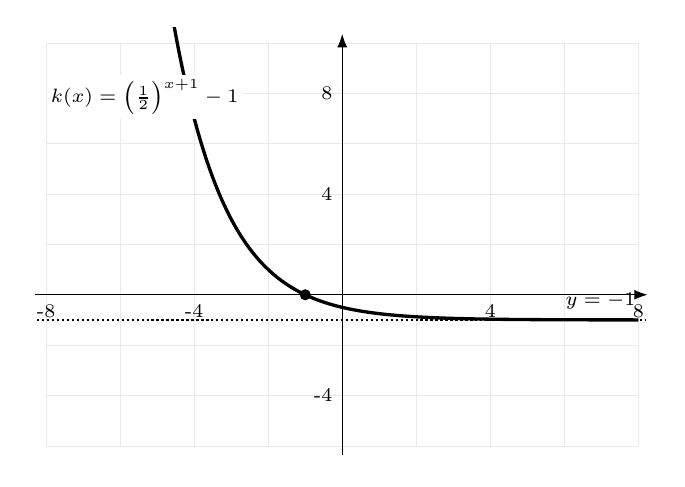
\begin{tikzpicture}[x=.47cm,y=.32cm,>=Latex]
\clip (-8.5,-6.5) rectangle (8.5,10.6);
\draw[step=2,gray!17,very thin] (-8,-6) grid (8,10);
\draw[->] (-8.3,0)--(8.25,0) node[right] {$x$};
\draw[->] (0,-6.35)--(0,10.35) node[above] {$y$};
\foreach \x in {-8,-4,4,8}{\node[below,font=\scriptsize] at (\x,0) {\x};}
\foreach \y in {-4,4,8}{\node[left,font=\scriptsize] at (0,\y) {\y};}
\draw[densely dotted,thick] (-8.25,-1)--(8.2,-1) node[above left,font=\scriptsize] {$y=-1$};
\draw[very thick,domain=-5:8,samples=130,smooth] plot (\x,{pow(0.5,\x+1)-1});
\fill (-1,0) circle (2pt);
\node[font=\scriptsize,anchor=north west,fill=white,inner sep=1.5pt] at (-8,8.75) {{$k(x)=\left(\frac{1}{2}\right)^{x+1}-1$}};
\end{tikzpicture}
\end{center}
\end{prikladReseniBox}
\poznamka{Vysvětlit rozdíl mezi $-2^x$ a $(-2)^x$. Druhý výraz nemá pro všechny reálné exponenty význam. Při kreslení používat dostatečný rozsah os; grafem není jen úsek mezi $x=-2$ a $x=2$.}
\Needspace{26\baselineskip}
\begin{prikladReseniBox}[title={Příklad 4}]
Sestroj graf $m(x)=-2\cdot2^{x-1}+3$:
\begin{enumerate}[label=\alph*)]
\item urči pořadí transformací;
\item vypočti $m(0)$ a $m(1)$;
\item urči asymptotu a obor hodnot.
\end{enumerate}
\tcblower
\begin{enumerate}[label=\alph*)]
\item Z $2^x$: posun doprava o 1, vynásobení funkčních hodnot $-2$, posun nahoru o 3.
\item $m(0)=2$, $m(1)=1$.
\item Asymptota $y=3$ a $H(m)=(-\infty;3)$; funkce klesá.
\end{enumerate}\begin{center}
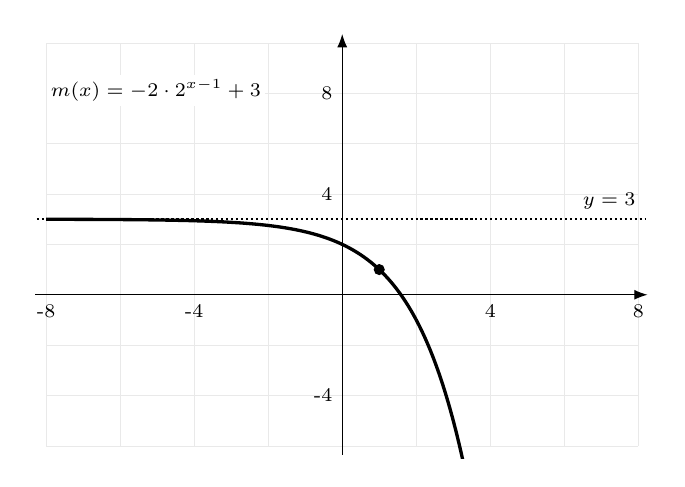
\begin{tikzpicture}[x=.47cm,y=.32cm,>=Latex]
\clip (-8.5,-6.5) rectangle (8.5,10.6);
\draw[step=2,gray!17,very thin] (-8,-6) grid (8,10);
\draw[->] (-8.3,0)--(8.25,0) node[right] {$x$};
\draw[->] (0,-6.35)--(0,10.35) node[above] {$y$};
\foreach \x in {-8,-4,4,8}{\node[below,font=\scriptsize] at (\x,0) {\x};}
\foreach \y in {-4,4,8}{\node[left,font=\scriptsize] at (0,\y) {\y};}
\draw[densely dotted,thick] (-8.25,3)--(8.2,3) node[above left,font=\scriptsize] {$y=3$};
\draw[very thick,domain=-8:5,samples=130,smooth] plot (\x,{-2*pow(2,\x-1)+3});
\fill (1,1) circle (2pt);
\node[font=\scriptsize,anchor=north west,fill=white,inner sep=1.5pt] at (-8,8.75) {{$m(x)=-2\cdot2^{x-1}+3$}};
\end{tikzpicture}
\end{center}
\end{prikladReseniBox}
\begin{zadaniReseniBox}[title={Samostatná práce 1}]
\begin{enumerate}[label=\alph*)]
\item Sestroj $f(x)=2^{x+2}-2$; urči posun, asymptotu a obor hodnot.
\item Sestroj $g(x)=3^{x-1}+1$; vyznač bod pro $x=1$.
\item Načrtni $h(x)=\left(\frac{1}{2}\right)^{x-2}+2$; urči monotónnost.
\item Načrtni $k(x)=2^x-4$; urči nulový bod.
\item Sestroj $m(x)=3-3^x$; urči průsečíky s osami.
\item Sestroj $n(x)=-2\cdot2^x+1$; urči obor hodnot.
\item Pro $p(x)=3^{x+2}-4$ urči $p(-2)$ a asymptotu.
\item Načrtni $q(x)=\left(\frac{1}{3}\right)^{x+1}-2$; označ body pro $x=-1,0$.
\item Vysvětli geometricky rozdíl mezi $2^{x-2}$ a $2^x-2$.
\item Z grafu $y=2^x$ odvoď předpis posunutý o 3 doleva a 2 nahoru.
\end{enumerate}
\tcblower
\begin{enumerate}[label=\alph*)]
\item Vlevo o 2 a dolů o 2, $y=-2$, $H=(-2;+\infty)$.
\item Vpravo o 1 a nahoru o 1; $g(1)=2$, $H=(1;+\infty)$.
\item Vpravo o 2 a nahoru o 2; funkce klesá, $H=(2;+\infty)$.
\item Dolů o 4; $2^x=4$, tedy $[2;0]$, asymptota $y=-4$.
\item Asymptota $y=3$, $m(0)=2$; nulový bod $3^x=3$ dává $[1;0]$.
\item Zrcadlení, svislé natažení a posun vzhůru; $H=(-\infty;1)$.
\item $p(-2)=1-4=-3$, asymptota $y=-4$.
\item $q(-1)=-1$, $q(0)=\frac{1}{3}-2=-\frac{5}{3}$; $y=-2$.
\item První posun doprava o 2; druhý dolů o 2.
\item $y=2^{x+3}+2$.
\end{enumerate}
\end{zadaniReseniBox}
\begin{zadaniReseniBox}[title={Rozšíření 1}]
\begin{enumerate}[label=\alph*)]
\item Najdi $b$, jestliže $f(x)=3^x+b$ prochází bodem $[2;12]$.
\item Urči asymptotu, obor hodnot a dva další body.
\end{enumerate}
\tcblower
\begin{enumerate}[label=\alph*)]
\item $9+b=12$, proto $b=3$.
\item $y=3$, $H=(3;+\infty)$; např. $[0;4]$, $[1;6]$.
\end{enumerate}
\end{zadaniReseniBox}
\begin{zadaniReseniBox}[title={Rozšíření 2}]
\begin{enumerate}[label=\alph*)]
\item Navrhni postup, jak získat graf $y=\left|2^{x-2}-4\right|$ z grafu $y=2^x$.
\item Urči přesně, kde se graf dotýká osy $x$, popiš obor hodnot a načrtni oba mezikroky.
\end{enumerate}
\tcblower
\begin{enumerate}[label=\alph*)]
\item Nejprve posun doprava o 2; potom dolů o 4. Část výsledného grafu pod osou $x$ odrazíme nahoru.
\item $2^{x-2}=4=2^2$ dává $x=4$, tedy bod $[4;0]$; $H=[0;+\infty)$. Levá větev se pro $x\to-\infty$ blíží k $y=4$.
\end{enumerate}
\end{zadaniReseniBox}
\begin{zadaniReseniBox}[title={Domácí úkol}]
\begin{enumerate}[label=\alph*)]
\item Pro $f(x)=2^{x+1}-4$ urči posuny, asymptotu a nulový bod.
\item Pro $g(x)=3-3^x$ urči $g(0)$, monotónnost a asymptotu.
\item Sestroj graf $y=2^{x-2}+1$ a označ tři jeho body.
\item Sestroj graf $y=\left(\frac{1}{2}\right)^{x+2}-2$; označ asymptotu.
\item Pro $m(x)=-3\cdot2^x+1$ urči obor hodnot a průsečík s osou $y$.
\item Pro $n(x)=4^x-3$ spočti $n(-1)$ a $n(1)$.
\item Vyjádři předpis grafu $y=3^x$ po posunu 2 doleva a 5 dolů.
\item Vyjádři předpis grafu $y=\left(\frac{1}{3}\right)^x$ po posunu 3 doprava.
\item Sestroj do jedné soustavy $y=2^x$ a $y=2^x+2$; popiš asymptoty.
\item Urči, proč $y=-2^x$ má obor hodnot $(-\infty;0)$, a načrtni graf.
\end{enumerate}
\tcblower
\begin{enumerate}[label=\alph*)]
\item Vlevo o 1, dolů o 4; asymptota $y=-4$, nulový bod $x=1$.
\item $g(0)=2$, klesá, asymptota $y=3$.
\item Asymptota $y=1$, např. $[1;\frac{3}{2}]$, $[2;2]$, $[3;3]$.
\item Asymptota $y=-2$, např. $[-2;-1]$, $[-1;-\frac{3}{2}]$, $[0;-\frac{7}{4}]$.
\item $H=(-\infty;1)$; $m(0)=-2$.
\item $n(-1)=\frac{1}{4}-3=-\frac{11}{4}$, $n(1)=1$.
\item $y=3^{x+2}-5$.
\item $y=\left(\frac{1}{3}\right)^{x-3}$.
\item Asymptoty $y=0$ a $y=2$; druhý graf je o 2 výše.
\item Veškeré hodnoty $2^x$ jsou kladné, po vynásobení $-1$ záporné; asymptota $y=0$.
\end{enumerate}
\end{zadaniReseniBox}
\poznamka{Po zadání domácího úkolu ještě připomenout, aby si žáci grafy skutečně narýsovali. Vhodná soustava pro většinu úloh: $x$ od $-8$ do $8$ a $y$ přibližně od $-6$ do $10$; u strmějších grafů měřítko upravit, křivku neomezovat na úsek $[-2;2]$.}
\end{document}
